\documentclass[12pt,halfparskip]{scrartcl}

\usepackage{../bodesuri}
\usepackage{float}

\newcommand{\dokumenttitel}{Qualitätssicherung}

\begin{document}

\title{\dokumenttitel}
\titlehead{
	\centering
	
\includegraphics[width=0.5 \textwidth, clip, trim = 0 7cm 0 0]{design/externes_design/bodesuri_plakat}
	\vspace{2cm}
}
\author{Danilo~Couto, Philippe~Eberli, \\ Pascal~Hobus, Reto~Schüttel, Robin~Stocker}
\maketitle
\newpage

\pagenumbering{roman}

\tableofcontents
\thispagestyle{plain}
\newpage

\pagenumbering{arabic}

\markright{Bodesuri -- \dokumenttitel}


\section{Coderichtlinien}\label{sub:coderichtlinien} % (fold)

Grundsätzlich folgen wir den "<Sun Coding Quidelines">. Zusätzlich gelten die folgenden Regeln:

\begin{itemize}
  \item Öffnende geschwungene Klammer (\texttt{\{}) auf gleicher Zeile
  \item Einrücken mit Tabulatoren, Formatieren mit Leerzeichen
  \item 1 Tabulator hat die Breite 4
  \item Maximal 80 Zeichen pro Zeile
  \item Sprache: Deutsch mit vernünftigen Ausnahmen (get und nicht gib...)
  \item Mit Javadoc kommentieren wo sinnvoll (z.\,B. keine Getter/Setter kommentieren)
  \item Paketnamen klein schreiben
  \item Copyright-Header\footnote{Die Möglichkeit einer Veröffentlichung des Projekts unter einer FOSS-Lizenz wird nach Abschluss des Projektes geprüft werden.} in allen Dateien:
    \begin{verbatim}
/* Copyright (c) 2007 Danilo Couto, Philippe Eberli,
 *                    Pascal Hobus, Reto Schüttel, Robin Stocker
 */
    \end{verbatim}
\end{itemize}


\paragraph{Beispielcode} (\texttt{----->} stellt einen Tabulator dar)

\begin{verbatim}
--->public void funktion(int erstens, int zweitens) {
--->--->if (erstens == zweitens) {
--->--->--->funktionZwei("Gleich");
--->--->} else {
--->--->--->funktionMitVielenArgumenten("Ungleich", erstens, zweitens,
--->--->--->                            undNochEinArgument);
--->--->}
--->}
\end{verbatim}

\section{Reviews} % (fold)
\label{sec:reviews}
Es wurden im Rahmen des Projektes verschiedene Code-Reviews durchgeführt. Sie dienten einerseits einer Qualitätskontrolle und andererseits fand dank ihnen auch ein verstärkter Know-How Transfer statt.

Ein Review dauerte in der Regel eine Stunde und wurde in wechselnden Paaren durchgeführt. Die dabei entstandenen Erkenntnissen und Aufgaben wurden im Wiki dokumentiert. Nachfolgend eine kurze Zusammenfassung der einzelnen Reviews

\subsubsection{Review Netzwerk - Pascal \& Reto}
\label{ssub:review_netzwerk_pascal_amp_reto}

\begin{itemize}
	\item Kleine Verbesserungen in den Netzwerk Klassen
	\item Verhalten bei Timeouts und Verbindungsfehlern diskutiert
	\item Weiteres Vorgehen für die Synchronisation zwischen Client und Server besprochen
\end{itemize}

\htmladdnormallink{http://www.bodesuri.ch/trac/wiki/Review\%202007-05-10\%20Pascal/Reto}{http://www.bodesuri.ch/trac/wiki/Review\%202007-05-10\%20Pascal/Reto}

\subsubsection{Problem Domain - Philippe \& Robin}
\label{ssub:problem_domain_philippe_amp_robin}

\begin{itemize}
	\item Kleine Refactorings (u.a. WegFeld umbenannt nacht NormalesFeld)
	\item Serialisierung vereinfacht
\end{itemize}

\htmladdnormallink{http://www.bodesuri.ch/trac/wiki/Review\%202007-06-25\%20Philippe/Robin}{http://www.bodesuri.ch/trac/wiki/Review\%202007-06-25\%20Philippe/Robin}

\subsubsection{GUI / Automaten Kommunikation - Danilo \& Pascal}
\label{ssub:gui_automaten_kommunikation_danilo_amp_pascal}

\begin{itemize}
	\item Kommunikation zwischen GUI und Automaten geplant
	\item Controller angeschaut und an einigen Stellen verbessert
\end{itemize}

\htmladdnormallink{http://www.bodesuri.ch/trac/wiki/Review\%202007-06-11\%20Pascal/Danilo}{http://www.bodesuri.ch/trac/wiki/Review\%202007-06-11\%20Pascal/Danilo}

\subsubsection{Automat - Reto \& Robin}
\label{ssub:automat_reto_amp_robin}

\begin{itemize}
	\item Synchronisation-Logik vereinfacht
	\item Neue Klasse Weg geplant die vom Regelsystem wie auch für die Wegmarkierung im UI verwendet werden kann
	\item Verschiedene kleinere Refactorings
\end{itemize}

\htmladdnormallink{http://www.bodesuri.ch/trac/wiki/Review\%202007-06-11\%20Reto/Robin}{http://www.bodesuri.ch/trac/wiki/Review\%202007-06-11\%20Reto/Robin}

\subsubsection{GUI - Danilo \& Philippe}
\label{ssub:gui_danilo_amp_philippe}

\begin{itemize}
	\item Lobby-View vereinfacht
	\item Setzen des Swing Look and Feels an einer zentralen Stelle
\end{itemize}

\htmladdnormallink{http://www.bodesuri.ch/trac/wiki/Review\%202007-06-22\%20Danilo/Philippe}{http://www.bodesuri.ch/trac/wiki/Review\%202007-06-22\%20Danilo/Philippe}

\subsubsection{User-Feeling - Philippe \& Robin}
\label{ssub:user_feeling_philippe_amp_robin}

\begin{itemize}
	\item Kleinere Bugs gefunden und behoben (z.\,B. falsche Reihenfolge)
	\item GUI-Handling an verschiedenen durch kleine Massnahmen verbessert
	\item Verschiedene Meldungen und Fehlermeldungen verbessert
\end{itemize}

\htmladdnormallink{http://www.bodesuri.ch/trac/wiki/Review\%202007-05-11\%20Philippe/Robin}{http://www.bodesuri.ch/trac/wiki/Review\%202007-05-11\%20Philippe/Robin}

\section{Auflösung zyklischer Abhängikeiten}
Im Laufe des Projektes zeigten sich im Design und im Code verschiedene zyklische Abhängigkeiten. Unter Verwendung des Tools \emph{Structure 101} konnten wir diese zyklischen Relationen einfach aufdecken und analysieren. Nachfolgend möchten wir dieses Vorgehen an einigen konkreten Beispielen aufzeigen.

\subsection{Zyklische Beziehung zwischen app.zugautomat und app.pd}

\begin{figure}[h]
	\centering
	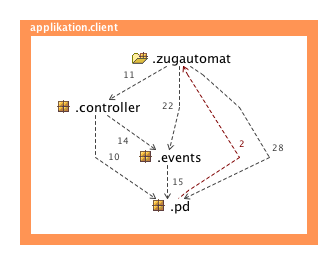
\includegraphics[width=0.5 \textwidth]{../design/probleme/zugautomat-client-pd}
	\caption{Zyklische Beziehung zwischen app.zugautomat und app.pd}
	\label{fig:zugautomat-client-pd}
\end{figure}

Der Zug-Automat (in Package app.zugautomat) und der Client teilen sich miteinander die Client-Problem-Domain (app.pd). Da aber diese zusätzlich noch eine Referenz auf den Zug-Automaten beinhaltet, ist die Beziehung zwischen den beiden Packages zyklisch. Ersichtlich auf der Abbildung~\vref{fig:zugautomat-client-pd}

\textbf{Lösung:} Die Referenz in app.pd muss nicht zwingend vom Typ \textbf{Zugautomat} sein, es genügt auch die Basiskasse \textbf{Automat}.

\subsection{Zyklische Beziehung zwischen den Klassen Feld2d und FeldMausAdpater}

Jedes Feld auf dem Spielbrett besitzt seinen eigenen FeldMouseAdapter welcher für die Verarbeitung der Click-Events zuständig ist. Dieser muss natürlich eine Referenz auf das Feld besitzen damit er etwaige Klicks an den Automaten melden kann. Das Feld (in Form der Klasse Feld2d) hingegen muss den FeldMouseAdapter als MouseAdapter registrieren und muss somit diesen auch als Referenz besitzen. Dies führt, wie auf der Abbildung ~\vref{fig:feld2d-feldmouseadapter} ersichtlich, zu einer zyklischen Beziehung zwischen den beiden Klassen.

\textbf{Lösung:} Das \textbf{Feld2d} muss gar nichts genaueres über den \textbf{FeldMouseadapter} wissen, es genügt für ihn zu wissen das es sich dabei um einen \textbf{MouseAdapter} handelt.

\begin{figure}[H]
	\centering
	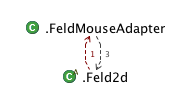
\includegraphics[width=0.3 \textwidth]{../design/probleme/feld2d-feldmouseadapter}
	\caption{Zyklische Beziehung zwischen den Klassen Feld2d und FeldMouseAdapter}
	\label{fig:feld2d-feldmouseadapter}
\end{figure}

\begin{figure}[H]
	\centering
	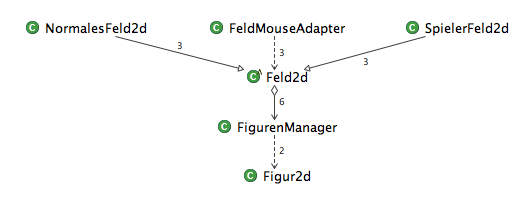
\includegraphics[width=0.8 \textwidth]{../design/probleme/feld2d-feldmouseadapter-nachher}
	\caption{Beziehung zwischen den Klassen Feld2d und FeldMouseAdapter nach Refactoring}
	\label{fig:feld2d-feldmouseadapter-nachher}
\end{figure}


\subsection{Zyklische Beziehungen in der Problem-Domain}
Die Problem-Domain war schon seit Beginn in verschiedenste zyklische Beziehungen verwickelt. Figuren kennen Felder, Felder kennen Figuren. Die Karten kennen die Regeln und umgekehrt. Wir fanden relativ spät im Projekt noch einen mögliche Verbesserung die aus folgenden Schritten bestand:

\begin{itemize}
	\item Neues Package \textbf{pd.spiel}
	\item \textbf{pd.brett}, \textbf{pd.spieler} und \textbf{pd.Spiel} ins Package \textbf{pd.spiel} verschieben
	\item Alle Klassen "<Zugeingabe*">  ins Package \textbf{pd.regelsystem} verschieben
	\item Die Methoden \textbf{Spieler\#kannZiehen()} und \textbf{Spieler\#moeglicheZuege()} in eine neue Klasse \textbf{pd.regelsystem.Regelsystem} verschieben
	\item \textbf{pd.karten} nach umbenennen \textbf{pd.regelsystem.karten}
\end{itemize}


\begin{figure}[H]
	\centering
	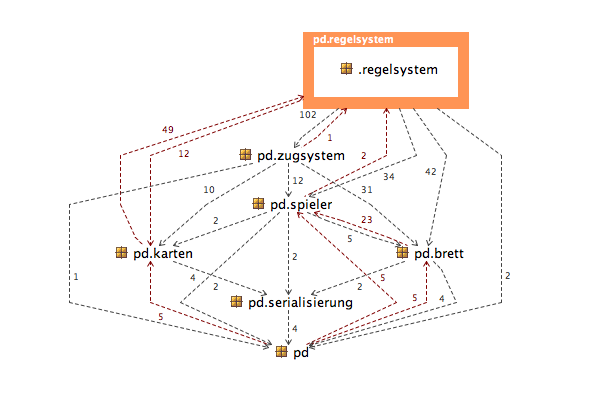
\includegraphics[width=0.8 \textwidth]{../design/probleme/package-level-vorher}
	\caption{Zyklische Beziehung PD}
\end{figure}

\begin{figure}[H]
	\centering
	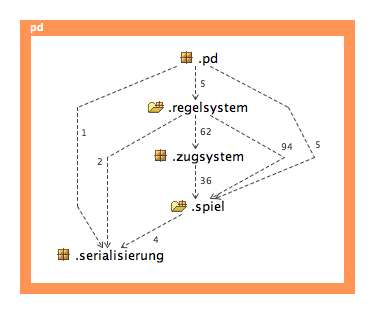
\includegraphics[width=0.5 \textwidth]{../design/probleme/package-level-nachher}
	\caption{Beziehung PD nach Refactoring}
\end{figure}

\newpage

\section{Tests}
\subsection{Voraussetzungen}
\begin{itemize}
	\item Die Tests werden alle im Vierspielermodus durchgeführt.
	\item Bots werden nur für Tests eingesetzt, welche sie reproduzierbar ein weiteres Mal durchlaufen können.
	\item Netzwerkverkehr und Netzwerkauslastung werden gezielt und reproduzierbar mit dem Tool iperf simuliert.
	\item Bei vermuteten TCP/IP-Problemen wird Wireshark als Sniffer verwendet und die aufgezeichneten Datenströme abgespeichert und dem Test eindeutig zugeordnet.
	\item Ein Test wird erst begonnen, wenn sein Vorgänger erfolgreich durchgeführt wurde.
\end{itemize}

\subsection{Vorbereitungen}
\paragraph{Vor allen Tests}\label{ssub:vorbereitungen_vor_allen_tests} 
	\begin{itemize}
		\item Auf den PCs, auf denen der Server und die Clients laufen, werden alle Firewalls deaktiviert oder die verwendeten Ports explizit freigeschaltet.
	\end{itemize}

\paragraph{Vor jeder Test-Iteration}\label{ssub:vorbereitungen_vor_jeder_testiteration}
	\begin{itemize}
		\item Testprotokoll zur Ausfüllung vorbereiten.
	\end{itemize}

\subsection{Nachbearbeitungen}\label{sec:nachbearbeitungen}
	\paragraph{Nach allen Tests}\label{ssub:nach_allen_tests}
		\begin{itemize}
			\item Alle Tests müssen erfolgreich absolviert worden sein.
			\item Alle Unit-Tests funktionieren (Green Bar).
		\end{itemize}

	\paragraph{Nach jeder Test-Iteration}\label{ssub:nach_jeder_test_iteration}
		\begin{itemize}
			\item Alle gefundenen Fehler wurden korrigiert.
			\item Alle Unit-Tests funktionieren (Green Bar).
			\item Testprotokoll wurde vollständig ausgefüllt.
		\end{itemize}		

\subsection{JUnit-Tests}
Die JUnit Tests, welche hauptsächlich die Dienste- und Problem-Domain-Klassen sowie weite Teile der Applikationsschicht abdecken wurden mit JavaDoc dokumentiert. Die UI-Schicht wird nicht explizit und nur punktuell durch JUnit-Tests abgedeckt. Sie wird hauptsächlich durch die Use-Case-Tests manuell getestet.

Details zu den JUnit Tests können aus der JavaDoc entnommen werden.

% TODO: ??: werden javadocs überhaupt generiert von den tests? (-reto)

\subsection{Systemtests}
\subsubsection{Use-Case Test: UC1 Spiel erstellen}
	\begin {tabular}{r | p{3cm} | p{8cm} | l}
		\toprule
		\textbf{UC} & \textbf{Beschreibung} & \textbf{Erwartetes Verhalten} & \textbf{Ergebnis} \\
		\midrule
		1, 2, 3 & Server-Start \newline erfolgreich & Der Server ist gestartet, funktioniert und ist betriebsbereit. & [Ok] \\
		 \cline{3-4} & & Für den Benutzer ist gut ersichtlich, dass der Server läuft und betriebsbereit ist. & [Ok] \\
		\midrule
		1, 2 & Mehrere Server-Instanzen & Es wird eine Fehlermeldung auf der Konsole ausgegeben und der Server beendet sich vollständig. & [Ok] \\
		\bottomrule
	\end{tabular}
	
\newpage

\subsubsection{UC2: Spiel beitreten}
	\begin {tabular}{r | p{3cm} | p{8cm} | l}
		\toprule
		\textbf{UC} & \textbf{Beschreibung} & \textbf{Erwartetes Verhalten} & \textbf{Ergebnis} \\
		\midrule
		1, 2, 3, 4 & Client verbunden & Der Client hat sich auf den Server verbunden und der Server kennt den Client. & [Ok] \\
		 \cline{3-4} & & Der Benutzer ist informiert worden, dass er dem Spiel erfolgreich beigetreten ist. In der Lobby kann er sich und seine Mitspieler erkennen und mit ihnen chatten. & [Ok] \\
		\midrule
		2a & Verbindung fehlgeschlagen & Der Benutzer wird vom System über das Scheitern benachrichtigt. Er ist gleich wieder in der Lage, einen neuen Verbindungsversuch zu unternehmen. & [Ok] \\
		\midrule
		2b & Server besetzt & Dem Benutzer wird mitgeteilt, dass der Server bereits voll ist. Das laufende Spiel wird nicht beeinflusst und der Client, der versucht hat auf den vollen Server zu verinbinden wird beendet. & [Ok] \\
		\midrule
		*a & Verbindung abgebrochen & Serverprozess beenden (Absturz simulieren). & [Ok]  \\
		\cline{3-4} & & Das Spiel wird mit einer Fehlermeldung abgebrochen. Alle Parteien werden über das Ende informiert. & [Ok] \\
		\midrule
		*a & Server und vier Clients starten. Spiel beginnen und einen Client beenden. & Server meldet Fehler, und wartet bis alle Clients stoppen Client melden im GUI den Fehler und beenden die Netzwerkverbindung. & [Ok] \\
		\midrule
		*a & Client (ohne Server) starten und verbinden. & Client meldet Fehler beim Verbindungsaufbau und kehrt zum Verndinden-Dialog zurück. & [Ok] \\
		\midrule
		*a & Server und Client starten. Client beenden. & Server und Clients beenden kontrolliert mit einer Fehlermeldung. & [Ok] \\
		\midrule
		*a & Server und zwei Clients starten, ein Client beenden. & Server meldet Fehler, und wartet bis alle Clients stoppen Client melden im GUI den Fehler und beenden die Netzwerkverbindung. & [Ok]  \\
		\bottomrule
	\end{tabular}
	
\subsubsection{UC3: Spiel spielen}
	\begin {tabular}{r | p{3cm} | p{9cm} | l}
		\toprule
		\textbf{UC} & \textbf{Beschreibung} & \textbf{Erwartetes Verhalten} & \textbf{Ergebnis} \\
		\midrule
		1 & Spielbrett initialisiert & Das Spielbrett ist initialisiert und auf allen Clients innerhalb der Zeitlimite von 3\,s synchronisiert. & [Ok] \\
		 \cline{3-4} & & Alle Clients und der Server befinden sich in einem wohldefinierten Zustand. & [Ok] \\
		\midrule
		2 & Karten erhalten & Der beteiligte Client hat die Spielkarten erhalten und visualisiert sie korrekt für den Spieler. & [Ok] \\
		\midrule
		3 & Karten für Tausch auswählen & Vom Benutzer ausgewählte Spielkarten sind visualisiert und als ausgewählt hervorgehoben. & [Ok] \\
		 \cline{3-4} & & Dem Spieler wird visuell mitgeteilt, dass das System bereit ist den Kartentausch abzuwickeln. & [Ok] \\
		\midrule
		4 & Karten-Tausch übermitteln & Die vom Benutzer getauschten Spielkarten sind an den Server übermittelt und auf dem Client (der die Spielkarten gesendet hat) nicht mehr vorhanden. & [Ok] \\
		 \cline{3-4} & & Der Client (der die Spielkarten gesendet hat) hat diejenigen Spielkarten vom Server empfangen, die der Partnerspieler zum Tausch an den Server übermittelt hatte. & [Ok] \\
		 \cline{3-4} & & Für den Spieler werden die Spielkarten nach dem Tausch korrekt visualisiert. & [Ok] \\
		\midrule
		5 & Spielzüge visualisieren & Benutzer kann keine spieleingreifende Eingaben tätigen. & [Ok] \\
		 \cline{3-4} & & Spielzüge werden korrekt auf dem Client visualisiert. & [Ok] \\
		 \cline{3-4} & & Client ist nach jedem Spielzug zu den anderen Clients synchronisiert. & [Ok] \\
		\midrule
	\end{tabular}
		
	\begin {tabular}{r | p{3cm} | p{9cm} | l}
		\toprule
		\textbf{UC} & \textbf{Beschreibung} & \textbf{Erwartetes Verhalten} & \textbf{Ergebnis} \\
		\midrule
		6 & Vorwärtszug erfassen & Der Spieler wählt das Start- und das Zielfeld aus und der Client validiert den Zug erfolgreich. & [Ok] \\
		\cline{3-4} & Rückwärtszug & Der Spieler wählt das Start- und das Zielfeld aus und der Client validiert den Zug erfolgreich. & [Ok] \\
		\cline{3-4} & Zug mit Joker & Nach anklicken der Joker-Karte wird eine Auswahl angezeigt, in der der Spieler die Karte wählen kann, mit der gespielt werden soll. Danach wählt der Spieler Start- und das Zielfeld aus und der Client validiert den Zug erfolgreich. & [Ok] \\
		\cline{3-4} & Aufteilbarer Zug & Der Spieler wählt das Start- und das Zielfeld für jede Figur aus, mit der er einen Teilzug durchführen möchte. & [Ok] \\
		\cline{3-4} & Aufteilbarer Zug (Spezialfall) & Wenn ein Spieler nur noch eine Figur hat, die noch nicht im Himmel steht und welche weniger als sieben Felder vom Himmel entfernt ist, so ist der Zug nicht auf seine Figur und der "<Rest"> der Teilzüge auf eine Figur des Partners anwendbar. Der Spieler kann in dieser Situation nur aufgeben. & [Ok] \\
		\cline{3-4} & Fressen fremder Figuren & Eine beliebige Figur (auch eine eigene) wird auf ihr Lagerfeld zurückgeschickt, sofern es nicht geschützt ist. & [Ok] \\
		\cline{3-4} & Ziehen mit Partnerfiguren & Wenn der Spieler all seine Figuren in den Himmel platzieren konnte, so kann er mit den Figuren des Partners fahren, als wären es seine eigenen. Alle Züge werden vom Client korrekt validiert. & [Ok] \\
		\cline{3-4} & Startzug & Die Figur wird vom Lagerfeld auf das Bankfeld des Spielers verschoben. & [Ok] \\
		\cline{3-4} & Figurentausch & Der Tausch wird sofort angezeigt und korrekt validiert. & [Ok] \\
		\cline{3-4} & Vorwärtszug (gesch. Bank) & Der Client registriert bei der Validierung einen Regelverstoss und informiert den Spieler. & [Ok] \\
		\cline{3-4} & Rückwärtszug (gesch. Bank) & Der Client registriert bei der Validierung einen Regelverstoss und informiert den Spieler. & [Ok] \\
		\cline{3-4} & Vorwärtszug in Himmel & Der erfasste Zug wird korrekt validiert, ausgeführt und dargestellt. & [Ok] \\
		\cline{3-4} & Vorwärtszug im Himmel & Der erfasste Zug wird korrekt validiert, ausgeführt und dargestellt. & [Ok] \\
		\cline{3-4} & Rückwärtszug im Himmel & Der Client registriert bei der Validierung einen Regelverstoss und informiert den Spieler. & [Ok] \\
		\bottomrule
	\end{tabular}
	
	\begin {tabular}{r | p{3cm} | p{8cm} | l}
		\toprule
		\textbf{UC} & \textbf{Beschreibung} & \textbf{Erwartetes Verhalten} & \textbf{Ergebnis} \\
		\midrule
		7, 8, 9 & Spielzug übermitteln & Spielzug ist vom Client validiert worden und gültig. & [Ok] \\
		 \cline{3-4} & & Spielzug ist an Server übermittelt. & [Ok] \\
		 \cline{3-4} & & Spielzug wird wird binnen drei Sekunden im Client visualisiert & [Ok] \\
		 \cline{3-4} & & Alle Clients haben den Spielzug visualisiert und sind synchronisiert. & [Ok] \\
		\midrule
		6a & Kein Karte spielbar & Dem Server wurde mitgeteilt, dass Spieler diese Runde nicht spielen kann. & [Ok] \\
		 \cline{3-4} & & Alle Clients sind synchronisiert. & [Ok] \\
		\midrule
		7a & Spielzug ungültig & Benutzer wird über ungültigen Zug benachrichtigt. & [Ok] \\
		 \cline{3-4} & & Benutzer weiss, dass er anderen Spielzug auswählen muss. & [Ok] \\
		\midrule
		9a a) & Spiel gewonnen & Auf allen Clients und dem Server ist das Spiel beendet. & [Ok] \\
		 \cline{3-4} & & Gewinner (-Partnerschaft) ist klar ersichtlich. & [Ok] \\
		\midrule
		9a b) & Spiel gewonnen & Der Server weiss, dass der Spieler fertig ist. & [Ok] \\
		 \cline{3-4} & & Spieler-Status ist auf allen Clients synchronisiert und für Spieler ersichtlich. & [Ok] \\
		 \cline{3-4} & & Der Spieler, der neu fertig ist, kann nun auch die Figuren des Partners bedienen (wenn er an der Reihe ist). & [Ok] \\
		\midrule
		*a) & Benutzer verlässt Spiel & Spiel wird auf allen Clients und dem Server beendet. & [Ok] \\
		\midrule
		*b) & Server nicht erreichbar & Benutzer wird vom System benachrichtigt. & [Ok] \\
		 \cline{3-4} & & Auf allen Clients wird eine Fehlermeldung angezeigt und das Spiel kontrolliert beendet. & [Ok] \\
		\bottomrule
	\end{tabular}
	
\subsection{Tests anhand der nichtfunktionalen Anforderungen}
	\begin {tabular}{l p{11cm} l}
		\toprule
		\textbf{Nr.} & \textbf{Beschreibung} & \textbf{Eingehalten} \\
		\midrule
		NF1 & Jeder Spielzug wird nach maximal 3 Sekunden visualisiert. Sprich der Zug wurde an den Server gesendet und vom Server wieder zurückerhalten. & [Ok] \\
		NF2 & Spielzustand ist nach jedem Spielzug in allen Clients und auf dem Server konsistent. & [Ok] \\
		NF3 & Inkonsistenz führt im Server und auf den Clients zu kontrolliertem Spielabbruch. & [Ok] \\
		NF4 & Es können nicht mehrere Spiele pro Server erstellt werden. & [Ok] \\
		NF5 & Ein Spiel kann nur mit der genauen Anzahl von vier Spielern gestartet werden. & [Ok] \\
		NF6 & Das GUI ist (bis auf die Verbindungsaufnahme) nur mit der Maus bedienbar. & [Ok] \\
		NF7 & Der Server sowie der Client ist uneingeschränkt auf den Plattformen Mac OS X 10.4, Windows XP SP2 und GNU/Linux verwendbar. & [Ok] \\
		NF8 & Weder für den Server noch für den Client ist eine Installation oder Konfiguration notwendig. & [Ok] \\
		NF9 & Ausser des Spielernamens und der Serverkonfiguration müssen keine Konfigurationen eingegeben werden. & [Ok] \\
		\bottomrule
	\end{tabular}

\section[Tester-Feedback]{Tester-Feedback\footnote{Die Namen der Tester wurden ananymisiert.}}

\subsection{Tester Schlomo}
\textbf{Wie alt bist du?}
\emph{21}

\textbf{Wie hat dir das Spiel gefallen? Dein genereller Eindruck?}
\emph{Die Spieleoberfläche ist sehr einladend und macht Lust auf das Spiel. Schönes Design und nette Implementation}

\textbf{Wie fandest du das Spielbrett und die umliegenden Kontrollelemente?}
\emph{Siehe oben.}

\textbf{Wie schnell konntest du dich mit dem Spiel zurecht finden?}
\emph{Auch ohne die Spielregeln zu lesen, findet man sich recht schnell zurecht. Einzig der Hinweis zum Kartentausch zu Beginn der Runde ist nicht so gut ersichtlich. Wenn man die Jokerkarte wählt und anschliessend eine beliebige Karte wählen darf, wird leider nicht mehr angezeigt, was für Züge mit der neuen Karte möglich wären.}

\textbf{Kanntest du Dog bereits?}
\emph{Nein, kannte nur "<Eile mit Weile">.}

\textbf{Hast du Fehler gefunden oder sonstige Unregelmässigkeiten?}
\emph{Beim aufteilen der Sprünge auf verschiedene Figuren (Karte 7) sind zum Teil etwas "<mühsame"> Situationen entstanden.}

\textbf{Was gefiel dir besonders gut?}
\emph{Design der Oberfläche (Implementation würde mir bestimmt auch gefallen, sah ich beim Spielen aber leider nicht).}

\textbf{Könntest du dir vorstellen im Internet gegen andere Spieler zu spielen?}
\emph{Ja, wäre interessant.}

\subsection{Testerin Katrin}
\textbf{Wie alt bist du?}
\emph{21}

\textbf{Wie hat dir das Spiel gefallen? Dein genereller Eindruck?}
\emph{Sehr gut, obwohl ich zuerst das Programm nicht kapiert habe...}

\textbf{Wie fandest du das Spielbrett und die umliegenden Kontrollelemente?}
\emph{Gut und übersichtlich dargestellt.}

\textbf{Wie schnell konntest du dich mit dem Spiel zurecht finden?}
\emph{Haha.. das dauerte schon seine Zeit, aber ich denke eher, dass das Problem bei mir lag.}

\textbf{Kanntest du Dog bereits?}
\emph{Jaja...}

\textbf{Falls ja, wie findest du unsere Umsetzung? Authentisch oder eher schwer nachvollziehbar?}
\emph{Gut, und sehr ähnlich wie beim Original. Obwohl ich leider noch nicht gegen "<wahre"> Gegner spielen konnte. Der Simulator ist einfach etwas blöde, daher war es nicht sooo schwierig.}

\textbf{Hast du Fehler gefunden oder sonstige Unregelmässigkeiten?}
\emph{Nö. Aber das liegt wahrscheindlich auch daran, dass ich den Blick für solche Dinge nicht habe.}

\textbf{Was gefiel dir besonders gut?}
\emph{Als ich endlich mal den Dreh raus hatte (war aber mein Problem), die Darstellung im Allgemeinen. Es ist übersichtlich.}

\textbf{Könntest du dir vorstellen im Internet gegen andere Spieler zu spielen?}
\emph{Ja. Aber nur Dog. Nicht Pokern oder solch ein Zeug.}

\subsection{Testerin Manuela}
\textbf{Wie alt bist du?}
\emph{22}

\textbf{Wie hat dir das Spiel gefallen? Dein genereller Eindruck?}
\emph{Das Spiel gefällt mir sehr gut! Leider sind die virtuellen Spieler ein wenig "<dumm">...}

\textbf{Wie fandest du das Spielbrett und die umliegenden Kontrollelemente?}
\emph{Übersichtlich, einfache Bedienung}

\textbf{Wie schnell konntest du dich mit dem Spiel zurecht finden?}
\emph{Sehr schnell, wahrscheinlich weil ich das Spiel schon kannte...}

\textbf{Kanntest du Dog bereits?}
\emph{Ja}

\textbf{Falls ja, wie findest du unsere Umsetzung? Authentisch oder eher schwer nachvollziehbar?}
\emph{Die Umsetzung ist sehr authentisch, ich habe mich auf Anhieb zurecht gefunden.}

\textbf{Hast du Fehler gefunden oder sonstige Unregelmässigkeiten?}
\emph{Nein, es funktionierte alles (habe bisher nur die Demo gespielt).}

\textbf{Was gefiel dir besonders gut?}
\emph{Ich finde es super, dass man zu viert spielen kann! (Leider ist dieses Brettspiel (noch) nicht so verbreitet, dass man einfach drei Mitspieler findet).}

\textbf{Könntest du dir vorstellen im Internet gegen andere Spieler zu spielen?}
\emph{Sicher, das Spiel gefällt mir viel besser als Ballerspiele etc.}

\subsection{Testerin Gabi}
\textbf{Wie alt bist du?}
\emph{21}

\textbf{Wie hat dir das Spiel gefallen? Dein genereller Eindruck?}
\emph{Sehr gut, es geht ein bisschen schnell, ich haben nie gewusst, wer jetzt anfängt oder wer die Karten gibt. Das Design gefällt mir sehr gut.}

\textbf{Wie fandest du das Spielbrett und die umliegenden Kontrollelemente?}
\emph{Sehr gut. Nur bei sieben hatte ich Mühe, das auf beide Kugeln aufzuteilen. Dass beim Joker die ganze Palette an Karten kommt, finde ich sehr hilfreich, auch dass bei jeder Karte steht, was man mit ihr machen muss.}

\textbf{Wie schnell konntest du dich mit dem Spiel zurecht finden?}
\emph{Recht schnell, liegt aber wahrscheinlich daran, dass ich das Spiel kenne. Man kann die sieben beim letzten Zug der eigenen Tötzel nicht auf die seines Partners übertragen. Im richtigen Dog geht dies jedoch.}

\textbf{Kanntest du Dog bereits?}
\emph{Ja.}

\textbf{Falls ja, wie findest du unsere Umsetzung? Authentisch oder eher schwer nachvollziehbar?}
\emph{Authentisch.}

\textbf{Hast du Fehler gefunden oder sonstige Unregelmässigkeiten?}
\emph{Oben erwähnt: 7 nicht auf Partner übertragbar bem letzten Zug.}

\textbf{Was gefiel dir besonders gut?}
\emph{Beim Joker die Kartenauflistung. Die Fehlermeldungen, also einfach, dass man auf die Fehler aufmerksam gemacht wird. Das Design, die Farben.}

\textbf{Könntest du dir vorstellen im Internet gegen andere Spieler zu spielen?}
\emph{Ja, aber nur gegen solche, die ich kenne. Sonst mache ich lieber mit Freunden ab und sehe sie direkt vor mir. Geht dann nicht so schnell und ist lustige, wenn man auch reden kann, ab und zu.}

\subsection{Tester Elias}
\textbf{Wie alt bist du?}
\emph{15}

\textbf{Wie hat dir das Spiel gefallen? Dein genereller Eindruck?}
\emph{Recht gut, der Computer war einfach zu besiegen.}

\textbf{Wie fandest du das Spielbrett und die umliegenden Kontrollelemente?}
\emph{Eigendlich gut.. aber der grüne teppich gefällt mir nicht so.}

\textbf{Wie schnell konntest du dich mit dem Spiel zurecht finden?}
\emph{Schnell.. nach ca. 5 min.}

\textbf{Kanntest du Dog bereits?}
\emph{Nein.}

\textbf{Hast du Fehler gefunden oder sonstige Unregelmässigkeiten?}
\emph{Nein.}

\textbf{Was gefiel dir besonders gut?}
\emph{Dass man nicht die einzelnen feldchen abzählen muss sondern das es dafür ein "<Zähler"> hat...:D ich fände es cool, wenn man Schwierigkeitsstufen gegen den computer einstellen könnte...}

\textbf{Könntest du dir vorstellen im Internet gegen andere Spieler zu spielen?}
\emph{Ja.}

\section{Bekannte Einschränkungen und Verbesserungsmöglichkeiten}
\subsection{Der Siebnerzug}
Der Siebnerzug ist aktuell so implementiert, dass man eine Figur nur genau einmal "<anfassen"> kann, das heisst sobald ein Teilzug gemacht wurde wird eine Geisterfigur auf das Zielfeld gesetzt und der Gesamtzug muss mit einer anderen Figur des gleichen Spielers weitergeführt werden.

Vom Spielgefühl her ist dies jedoch nicht das korrekte Verhalten. Logisch gesehen gibt es keinen Grund, warum man dies so einschränken sollte. Auch von den Spielregeln her ist es erlaubt, eine Figur beim Siebnerzug mehrmals zu bewegen. Dies bestätigt auch ein Testerfeedback einer sehr erfahrenen Dog-Spielerin, die dieses Verhalten relativ schnell erkannt und bemängelt hat.

Als Verbesserung würde es sich anbieten, den Siebnerzug bereits in der Problem-Domain speziell zu behandeln, um ein "<Rollback"> einer bereits durchgeführten Aktion durchführen zu können. So würde jeder Teilzug als separater Zug ablaufen. Würde ein Zug dann jedoch nicht mehr validiert werden können, wäre es möglich alle ausgeführten Aktionen wieder rückgängig zu machen.

\subsection{Partnerschaften}
Im Spiel werden die Partnerschaften fix durch den Server vorgeschrieben. Für den Spielspass ist dies nicht die optimale Lösung, da es sich bei Dog ja um ein Gesellschaftsspiel handelt. Wünschenswert wäre, wenn ein Spieler schon in der Lobby bestimmen kann, mit wem er eine Partnerschaft eingehen möchte.

\subsection{Der Computergegner (Bot)}
Der aktuell implementierte "<StupidBot"> stellt für die meisten Spieler keinen würdigen Gegner dar. Er wählt aus allen möglichen Zügen, die ihm zur Verfügung stehen einen zufälligen aus und verfolgt somit keine gezielte Strategie. Zu Beginn war dieser Bot auch lediglich zu Testzwecken gedacht. Da er aber sehr einfach zu implementieren war und uns doch gezeigt hatte, dass er das Spiel unter Anwendung aller möglichen Regeln zu Ende spielen konnte, haben wir beschlossen ihn in eine Demo zu integrieren um so einen Einzelspielermodus zu ermöglichen.

Da der Bot auf der Gesamtlösung aufsetzt -- er interagiert mit dem System anstelle des Spielers -- kann er in Zukunft einfach verändert werden, ohne dass etwaige Abhängigkeiten berücksichtigt werden müssen. Wir haben auch für intelligentere Bots schon einige Ideen angedacht:
\begin{itemize}
	\item Bot-Klasse als Interface oder abstrakte Klasse extrahieren.
	\item Bots implementieren verschiedene Strategien (z.\,B. aggressiv oder passiv).
	\item Mehrere Bot-Implementierungen sind möglich.
\end{itemize}

Einen intelligenten Bot zu programmieren ist jedoch nicht so einfach wie es auf den ersten Blick aussieht. Um aus seinen möglichen Zügen den Besten auszuwählen muss er verschiedene Varianten durchprobieren und vergleichen können. Er muss z.\,B. bei jedem Zug verschiedene Faktoren berücksichtigen:
\begin{itemize}
	\item Welchem Spieler gehört eine Figur?
	\item Ist es besser einen Gegner heimzuschicken, bevor dieser in seinen Himmel ziehen kann?
	\item Ist es besser, dem Partner eine Karte zuzuschieben und dafür eigene Nachteile zu kassieren?
	\item Werden beim aktuellen Zug Figuren von mir oder meinem Partner gefressen?
	\item Welche Karte soll am Anfang einer Runde getauscht werden?
	\item Wie ist die Situation der Figuren in zukünftigen Runden? (Vorhersage)
\end{itemize}

Um eine Strategie statisch abzubilden hatten wir schon grob einige Ideen aufgeschrieben:
\begin{itemize}
	\item Strategien können gewichtet werden.
	\item Bots können die Strategie zur Laufzeit ändern.
	\item Die Gewichtungen der verschiedenen Strategien werden durch das Verhalten der Gegner immer neu angepasst um die optimale Strategie zu finden.
\end{itemize}

Diese Thematik wird von uns sicherlich noch weiterverfolgt und auch implementiert werden, da es uns sehr interessiert.

\subsection{Steuerung und Konfiguration des Servers}
Der Server ist so implementiert worden, dass er für einen ungeübten Computerbenutzer möglichst einfach in der Handhabung ist. Aktuell ist es so gelöst, dass ein Spieler den Server "<per Doppelklick"> startet und ihn als normale Anwendung in der Taskleiste sieht. Dies funktioniert in den meisten Fällen sehr gut und ist für unsere Zwecke völlig ausreichend. Für den Benutzer gäbe es natürlich auch konfortablere Lösungen. Einige Ideen möchten wir hier kurz anreissen:
\begin{itemize}
	\item Rudimentäres GUI zur Konfiguration (z.\,B. die Portnummer).
	\item Konsole zur Anzeige aktueller Infos und Fehlermeldungen.
	\item Buttons zum Beenden des Servers.
	\item Server aus Client startbar/steuerbar.
\end{itemize}

\end{document}
